\documentclass{article}
\usepackage{amsmath}
\usepackage{amssymb}
\usepackage{mathtools}
\usepackage{tcolorbox}
\usepackage{graphicx}
\usepackage[colorlinks=true, linkcolor=blue]{hyperref}

\def\R{\mathbb{R}}

\DeclarePairedDelimiter\abs{\lvert}{\rvert}%

\title{Exercise 2}
\author{Daniel Gallo}
\date{October 2020}

\begin{document}
    \maketitle
    \section*{21.11 - Standard facts about infinite series}
    \begin{tcolorbox}[title=Exercise a]
        \label{21.11a}
        Show that if $(s_n)$ is a bounded sequence of real numbers and $s_n \leq s_{n + 1}$ for each $n$, then $(s_n)$ converges.
    \end{tcolorbox}
    \noindent
    The sequence $(s_n)$ will converge to $s = \sup\left\{s_n\right\}$, since for every $\epsilon > 0$ there exists $N$ such that $s_N > s - \epsilon$. If it didn't exist, $s - \epsilon$ would be an upper bound of $(s_n)$, which contradicts the definition of $s$. Since $(s_n)$ is increasing and $s$ is its supremum, $\forall n \geq N$ we have $\abs{s - s_n} < \epsilon$.
    \begin{tcolorbox}[title=Exercise b]
        \label{21.11b}
        Let $(a_n)$ be a sequence of real numbers and define
        \begin{equation*}
            s_n = \sum_{i=1}^n{a_i}
        \end{equation*}
        If $s_n \rightarrow s$, we say that the infinite series
        \begin{equation*}
            \sum_{i=1}^\infty{a_i}
        \end{equation*}
        converges to s. Show that if $\sum{a_i}$ converges to $s$ and $\sum{b_i}$ converges to $t$ then $\sum{ca_i + b_i}$ converges to $cs + t$.
    \end{tcolorbox}
    \noindent
    Since $\sum{a_i}$ converges to $s$, and $\sum{b_i}$ converges to $t$, for every epsilon we can find $N$ such that for every $n \geq N$
    \begin{equation*}
        \abs*{s - \sum_{i=1}^n{a_i}} < \epsilon \qquad \text{and} \qquad \abs*{t - \sum_{i=1}^n{b_n}} < \epsilon
    \end{equation*}
    Now we will prove that $\sum{ca_i + b_i}$ converges to $cs + t$ by definition.
    \begin{equation*}
        \abs*{cs+t - \sum_{i=1}^n{\left(ca_i + b_i\right)}} = \abs*{c\left(s - \sum_{i=1}^n{a_i}\right) + \left(\sum_{i=1}^n{b_i}\right)} < \epsilon(1 + \abs{c})
    \end{equation*}
    \begin{tcolorbox}[title=Exercise c]
        \label{21.11c}
        Prove the \textbf{comparison test} for infinite series: If $\abs{a_i} \leq b_i$ for each $i$, and if the series $\sum{b_i}$ converges, then the series $\sum{a_i}$ converges.
    \end{tcolorbox}
    \noindent
    First we'll prove that $\sum{\abs{a_i}}$ converges. It is clear that $\sum{\abs{a_i}}$ is bounded:
    \begin{equation*}
        \sum_{i=1}^\infty{\abs{a_i}} \leq \sum_{i=1}^\infty{b_i} < \infty
    \end{equation*}
    It is also a monotonic sequence, since $\abs{a_i} \geq 0$, so we can conclude by \hyperref[21.11a]{a} that $\sum{\abs{a_i}}$ converges. Using a similar reasoning we can prove that $\sum{\abs{a_i} + a_i}$ converges. 
    \begin{equation*}
        -\abs{a_i} \leq a_i \leq \abs{a_i} \quad \Rightarrow \quad 0 \leq \abs{a_i} + a_i \leq 2\abs{a_i}
    \end{equation*}
    $\sum{\abs{a_i} + a_i}$ is increasing (each term is greater or equal to zero) and the infinite sum is bounded by $2\sum{\abs{a_i}}$, which is finite. Thus, we conclude that $\sum{\abs{a_i} + a_i}$ converges. Now we just have to use \hyperref[21.11b]{b} to show that $\sum{(-1)\abs{a_i} + \abs{a_i} + a_i} = \sum{a_i}$ converges. 
    \begin{tcolorbox}[title=Exercise d]
        Given a sequence of functions $f_n \colon X \to \R$ let
        \begin{equation*}
            s_n(x) = \sum_{i=1}^n{f_i(x)}
        \end{equation*}
        Prove the \textbf{Weierstrass M-test} for uniform convergence: If $\abs{f_i(x)} \leq M_i$ for all $x \in X$ and all $i$, and if the series $\sum{M_i}$ converges, then the sequence $(s_n)$ converges uniformly to a function s.
    \end{tcolorbox}
    \noindent
    We want to show that for every $\epsilon$ there exists a $N$ such that for every $n > N$, the following holds:
    \begin{equation*}
        \abs{s(x) - s_n(x)} < \epsilon \quad \forall x \in X
    \end{equation*}
    \begin{align*}
        \abs{s(x) - s_n(x)} &= \abs*{\sum_{i=1}^\infty{f_i(x)} - \sum_{i=n}^\infty{f_i(x)}} \\
        &= \abs*{\sum_{i=n+1}^\infty{f_i(x)}} \\
        &\leq \sum_{i=n+1}^\infty{\abs{f_i(x)}} & \text{by the triangle inequality} \\
        &\leq \sum_{i=n+1}^\infty{\abs{M_i}} \rightarrow 0
    \end{align*}
    Since $\sum{M_i}$ converges, we can always choose $N$ big enough so $\sum_{i=n+1}^\infty{\abs{M_i}} < \epsilon$.
    
    \section*{26.7}
    \begin{tcolorbox}[title=Statement]
        If $Y$ is compact, then the projection $\pi_1\colon X \times Y \to X$ is a closed map.
    \end{tcolorbox}
    \noindent
    Let $C$ be a closed map in $X \times Y$. We want to prove that $\pi_1(C)$ is closed. As usually, we will show that $X - \pi_1(C)$ is an open set in $X$ saying that for every $x \in X - \pi_1(C)$ there exists a neighborhood $U$ such that $U \subset X - \pi_1(C)$. 
    \\
    Let $x \in X - \pi_1(C)$. By definition, we know that the line $\{(x, y) \mid y \in Y\}$ does not intersect $C$. Because of that, and taking into account that $C$ is closed, for every $y$ we can consider neighborhoods that won't intersect $C$ of the form $U_y \times V_y$. Since $Y$ is compact and $V_y$ covers $Y$, we can extract a finite subcovering $\{V_1, ..., V_n\}$. Let $U$ be defined as follows:
    \begin{equation*}
        U = \bigcap_{i=1}^{n}{U_i}
    \end{equation*}
    $U$ is an open set (finite intersection of sets) that doesn't intersect $\pi_1(C)$. We will prove this by contradiction. Assume $x' \in \pi_1(C) \cap U$. Then, there exists $(x', y') \in C$. But since $x' \in U$, there exists a neighborhood containing $(x', y')$ separating in from $C$.
    
    \section*{26.8}
    \begin{tcolorbox}[title=Statement]
        Let $f\colon X \to Y$ and let $Y$ be compact Hausdorff. Then $f$ is continuous if and only if the \textbf{graph} of $f$,
        \begin{equation*}
            G_f = \{x \times f(x) \mid x \in X\}
        \end{equation*}
        is closed in $X \times Y$
    \end{tcolorbox}
    \noindent
    First we'll prove that if $f$ is continuous, the graph is closed. 
    \begin{center}
    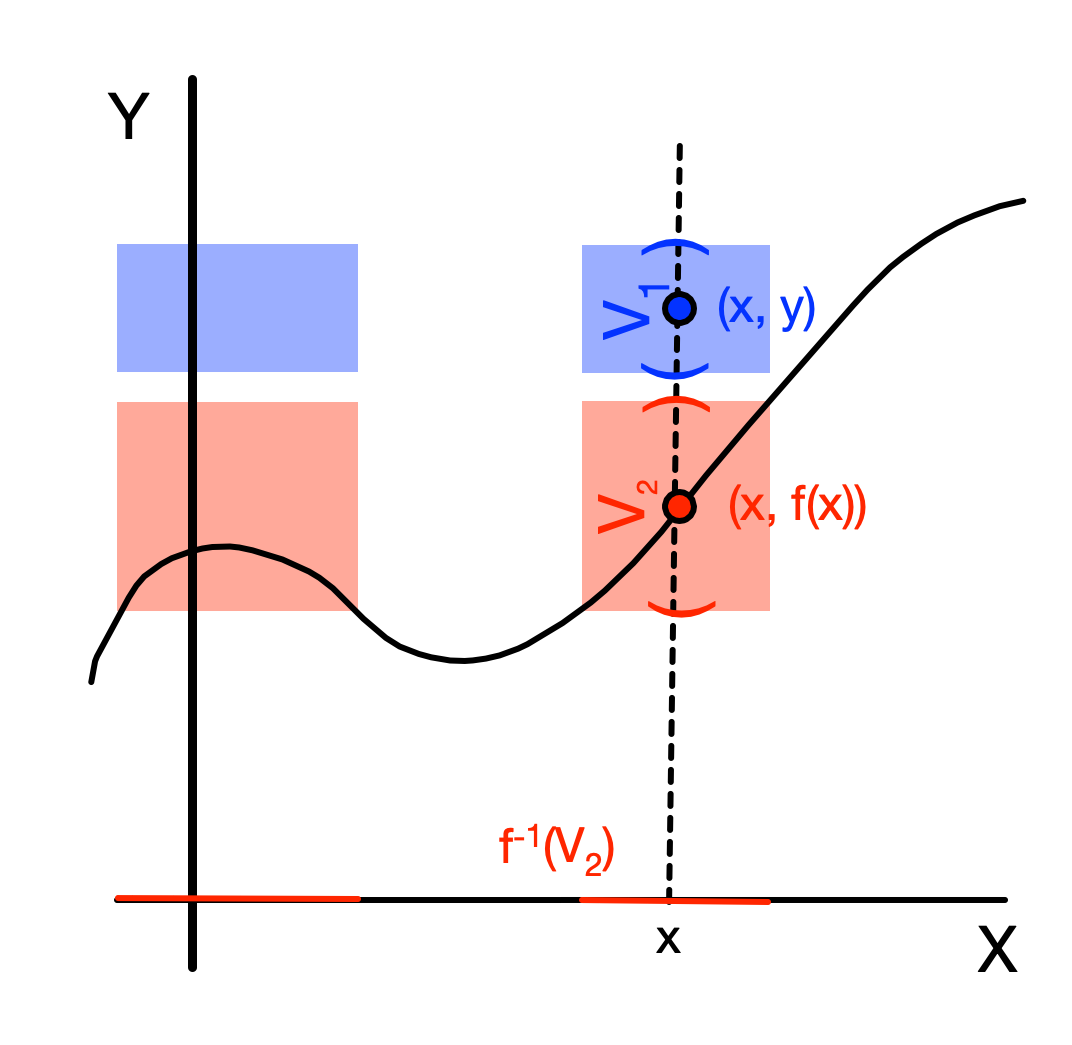
\includegraphics[width=0.6\textwidth]{diagram.png}
    \end{center}
    As we usually do, we'll take $(x, y) \notin G_f$ and we'll prove that there is an open set that contains $(x, y)$ and is contained on the complement of $G_f$. Since $y \neq f(x)$ and $Y$ is Hausdorff we can find $V_1$ and $V_2$ disjoint neighborhoods of $y$ and $f(x)$, respectively. We now use the fact that $f$ is continuous to obtain $f^{-1}(V_2)$, an open subset of $X$. The open set we were looking for is $f^{-1}(V_2) \times V_1$, which is painted blue in the diagram. The only thing we still have to prove is that it doesn't intersect the graph. If $(a, f(a))$ were in $f^{-1}(V_2) \times V_1$, $f(a)$ would be in $V_1$ and $V_2$. This is not possible since we chose $V_1$ and $V_2$ disjoint.
    \par
    \noindent
    \\
    Now we'll prove that if the graph of $f$ is closed, $f$ is continuous. To do so, consider $V$ open in $Y$ and let's prove that $f^{-1}(V)$ is open in $X$. 
    \begin{align*}
        \overline{f^{-1}(V)} &= \{x \mid f(x) \notin V\} \\
        &= \pi_1((x, f(x)) \mid f(x) \notin V) \\
        &= \pi_1((X \times (Y - V)) \cap G_f)
    \end{align*}
    Consider $f(x) \in V$ (if $V$ was empty, its preimage would be empty as well). Since $X$ is closed (it's complement is the empty set, which is open) and $Y - V$ is closed too (it's complement is $V$, which is open), $X \times (Y - V)$ is closed as well. Because the intersection of closed sets is closed we get to the conclusion that $G_f \cap (X \cap (Y - V))$ is closed. Using now exercise 26.7, we get that $\pi_1(G_f \cap (X \cap (Y - V))) = \overline{f^{-1}(V)}$ is closed. Thus, $f^{-1}(V)$ is open, as we wanted. 
\end{document}